\documentclass[1p]{elsarticle_modified}
%\bibliographystyle{elsarticle-num}

%\usepackage[colorlinks]{hyperref}
%\usepackage{abbrmath_seonhwa} %\Abb, \Ascr, \Acal ,\Abf, \Afrak
\usepackage{amsfonts}
\usepackage{amssymb}
\usepackage{amsmath}
\usepackage{amsthm}
\usepackage{scalefnt}
\usepackage{amsbsy}
\usepackage{kotex}
\usepackage{caption}
\usepackage{subfig}
\usepackage{color}
\usepackage{graphicx}
\usepackage{xcolor} %% white, black, red, green, blue, cyan, magenta, yellow
\usepackage{float}
\usepackage{setspace}
\usepackage{hyperref}

\usepackage{tikz}
\usetikzlibrary{arrows}

\usepackage{multirow}
\usepackage{array} % fixed length table
\usepackage{hhline}

%%%%%%%%%%%%%%%%%%%%%
\makeatletter
\renewcommand*\env@matrix[1][\arraystretch]{%
	\edef\arraystretch{#1}%
	\hskip -\arraycolsep
	\let\@ifnextchar\new@ifnextchar
	\array{*\c@MaxMatrixCols c}}
\makeatother %https://tex.stackexchange.com/questions/14071/how-can-i-increase-the-line-spacing-in-a-matrix
%%%%%%%%%%%%%%%

\usepackage[normalem]{ulem}

\newcommand{\msout}[1]{\ifmmode\text{\sout{\ensuremath{#1}}}\else\sout{#1}\fi}
%SOURCE: \msout is \stkout macro in https://tex.stackexchange.com/questions/20609/strikeout-in-math-mode

\newcommand{\cancel}[1]{
	\ifmmode
	{\color{red}\msout{#1}}
	\else
	{\color{red}\sout{#1}}
	\fi
}

\newcommand{\add}[1]{
	{\color{blue}\uwave{#1}}
}

\newcommand{\replace}[2]{
	\ifmmode
	{\color{red}\msout{#1}}{\color{blue}\uwave{#2}}
	\else
	{\color{red}\sout{#1}}{\color{blue}\uwave{#2}}
	\fi
}

\newcommand{\Sol}{\mathcal{S}} %segment
\newcommand{\D}{D} %diagram
\newcommand{\A}{\mathcal{A}} %arc


%%%%%%%%%%%%%%%%%%%%%%%%%%%%%5 test

\def\sl{\operatorname{\textup{SL}}(2,\Cbb)}
\def\psl{\operatorname{\textup{PSL}}(2,\Cbb)}
\def\quan{\mkern 1mu \triangleright \mkern 1mu}

\theoremstyle{definition}
\newtheorem{thm}{Theorem}[section]
\newtheorem{prop}[thm]{Proposition}
\newtheorem{lem}[thm]{Lemma}
\newtheorem{ques}[thm]{Question}
\newtheorem{cor}[thm]{Corollary}
\newtheorem{defn}[thm]{Definition}
\newtheorem{exam}[thm]{Example}
\newtheorem{rmk}[thm]{Remark}
\newtheorem{alg}[thm]{Algorithm}

\newcommand{\I}{\sqrt{-1}}
\begin{document}

%\begin{frontmatter}
%
%\title{Boundary parabolic representations of knots up to 8 crossings}
%
%%% Group authors per affiliation:
%\author{Yunhi Cho} 
%\address{Department of Mathematics, University of Seoul, Seoul, Korea}
%\ead{yhcho@uos.ac.kr}
%
%
%\author{Seonhwa Kim} %\fnref{s_kim}}
%\address{Center for Geometry and Physics, Institute for Basic Science, Pohang, 37673, Korea}
%\ead{ryeona17@ibs.re.kr}
%
%\author{Hyuk Kim}
%\address{Department of Mathematical Sciences, Seoul National University, Seoul 08826, Korea}
%\ead{hyukkim@snu.ac.kr}
%
%\author{Seokbeom Yoon}
%\address{Department of Mathematical Sciences, Seoul National University, Seoul, 08826,  Korea}
%\ead{sbyoon15@snu.ac.kr}
%
%\begin{abstract}
%We find all boundary parabolic representation of knots up to 8 crossings.
%
%\end{abstract}
%\begin{keyword}
%    \MSC[2010] 57M25 
%\end{keyword}
%
%\end{frontmatter}

%\linenumbers
%\tableofcontents
%
\newcommand\colored[1]{\textcolor{white}{\rule[-0.35ex]{0.8em}{1.4ex}}\kern-0.8em\color{red} #1}%
%\newcommand\colored[1]{\textcolor{white}{ #1}\kern-2.17ex	\textcolor{white}{ #1}\kern-1.81ex	\textcolor{white}{ #1}\kern-2.15ex\color{red}#1	}

{\Large $\underline{11a_{292}~(K11a_{292})}$}

\setlength{\tabcolsep}{10pt}
\renewcommand{\arraystretch}{1.6}
\vspace{1cm}\begin{tabular}{m{100pt}>{\centering\arraybackslash}m{274pt}}
\multirow{5}{120pt}{
	\centering
	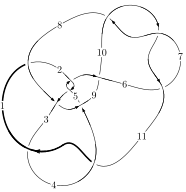
\includegraphics[width=112pt]{../../../GIT/diagram.site/Diagrams/png/541_11a_292.png}\\
\ \ \ A knot diagram\footnotemark}&
\allowdisplaybreaks
\textbf{Linearized knot diagam} \\
\cline{2-2}
 &
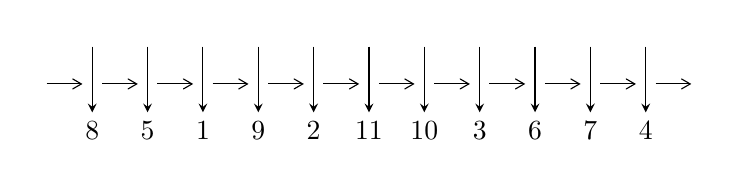
\begin{tikzpicture}[x=20pt, y=17pt]
	% nodes
	\node (C0) at (0, 0) {};
	\node (C1) at (1, 0) {};
	\node (C1U) at (1, +1) {};
	\node (C1D) at (1, -1) {8};

	\node (C2) at (2, 0) {};
	\node (C2U) at (2, +1) {};
	\node (C2D) at (2, -1) {5};

	\node (C3) at (3, 0) {};
	\node (C3U) at (3, +1) {};
	\node (C3D) at (3, -1) {1};

	\node (C4) at (4, 0) {};
	\node (C4U) at (4, +1) {};
	\node (C4D) at (4, -1) {9};

	\node (C5) at (5, 0) {};
	\node (C5U) at (5, +1) {};
	\node (C5D) at (5, -1) {2};

	\node (C6) at (6, 0) {};
	\node (C6U) at (6, +1) {};
	\node (C6D) at (6, -1) {11};

	\node (C7) at (7, 0) {};
	\node (C7U) at (7, +1) {};
	\node (C7D) at (7, -1) {10};

	\node (C8) at (8, 0) {};
	\node (C8U) at (8, +1) {};
	\node (C8D) at (8, -1) {3};

	\node (C9) at (9, 0) {};
	\node (C9U) at (9, +1) {};
	\node (C9D) at (9, -1) {6};

	\node (C10) at (10, 0) {};
	\node (C10U) at (10, +1) {};
	\node (C10D) at (10, -1) {7};

	\node (C11) at (11, 0) {};
	\node (C11U) at (11, +1) {};
	\node (C11D) at (11, -1) {4};
	\node (C12) at (12, 0) {};

	% arrows
	\draw[->,>={angle 60}]
	(C0) edge (C1) (C1) edge (C2) (C2) edge (C3) (C3) edge (C4) (C4) edge (C5) (C5) edge (C6) (C6) edge (C7) (C7) edge (C8) (C8) edge (C9) (C9) edge (C10) (C10) edge (C11) (C11) edge (C12) ;	\draw[->,>=stealth]
	(C1U) edge (C1D) (C2U) edge (C2D) (C3U) edge (C3D) (C4U) edge (C4D) (C5U) edge (C5D) (C6U) edge (C6D) (C7U) edge (C7D) (C8U) edge (C8D) (C9U) edge (C9D) (C10U) edge (C10D) (C11U) edge (C11D) ;
	\end{tikzpicture} \\
\hhline{~~} \\& 
\textbf{Solving Sequence} \\ \cline{2-2} 
 &
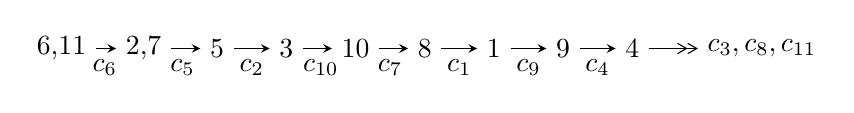
\begin{tikzpicture}[x=25pt, y=7pt]
	% node
	\node (A0) at (-1/8, 0) {6,11};
	\node (A1) at (17/16, 0) {2,7};
	\node (A2) at (17/8, 0) {5};
	\node (A3) at (25/8, 0) {3};
	\node (A4) at (33/8, 0) {10};
	\node (A5) at (41/8, 0) {8};
	\node (A6) at (49/8, 0) {1};
	\node (A7) at (57/8, 0) {9};
	\node (A8) at (65/8, 0) {4};
	\node (C1) at (1/2, -1) {$c_{6}$};
	\node (C2) at (13/8, -1) {$c_{5}$};
	\node (C3) at (21/8, -1) {$c_{2}$};
	\node (C4) at (29/8, -1) {$c_{10}$};
	\node (C5) at (37/8, -1) {$c_{7}$};
	\node (C6) at (45/8, -1) {$c_{1}$};
	\node (C7) at (53/8, -1) {$c_{9}$};
	\node (C8) at (61/8, -1) {$c_{4}$};
	\node (A9) at (10, 0) {$c_{3},c_{8},c_{11}$};

	% edge
	\draw[->,>=stealth]	
	(A0) edge (A1) (A1) edge (A2) (A2) edge (A3) (A3) edge (A4) (A4) edge (A5) (A5) edge (A6) (A6) edge (A7) (A7) edge (A8) ;
	\draw[->>,>={angle 60}]	
	(A8) edge (A9);
\end{tikzpicture} \\ 

\end{tabular} \\

\footnotetext{
The image of knot diagram is generated by the software ``\textbf{Draw programme}" developed by Andrew Bartholomew(\url{http://www.layer8.co.uk/maths/draw/index.htm\#Running-draw}), where we modified some parts for our purpose(\url{https://github.com/CATsTAILs/LinksPainter}).
}\phantom \\ \newline 
\centering \textbf{Ideals for irreducible components\footnotemark of $X_{\text{par}}$} 
 
\begin{align*}
I^u_{1}&=\langle 
14579744602 u^{24}+15331471056 u^{23}+\cdots+396477743843 b-332846474137,\\
\phantom{I^u_{1}}&\phantom{= \langle  }362005963341 u^{24}-27656036296 u^{23}+\cdots+1585910975372 a-1558403855541,\\
\phantom{I^u_{1}}&\phantom{= \langle  }u^{25}+11 u^{23}+\cdots+5 u-4\rangle \\
I^u_{2}&=\langle 
8 u^{20} a-2 u^{20}+\cdots- a-2,\;-2 u^{20} a+3 u^{20}+\cdots+a^2+10,\;u^{21}+u^{20}+\cdots- u-1\rangle \\
I^u_{3}&=\langle 
b+1,\;2 u^2+2 a-2 u+5,\;u^3- u^2+2 u-1\rangle \\
\\
\end{align*}
\raggedright * 3 irreducible components of $\dim_{\mathbb{C}}=0$, with total 70 representations.\\
\footnotetext{All coefficients of polynomials are rational numbers. But the coefficients are sometimes approximated in decimal forms when there is not enough margin.}
\newpage
\renewcommand{\arraystretch}{1}
\centering \section*{I. $I^u_{1}= \langle 1.46\times10^{10} u^{24}+1.53\times10^{10} u^{23}+\cdots+3.96\times10^{11} b-3.33\times10^{11},\;3.62\times10^{11} u^{24}-2.77\times10^{10} u^{23}+\cdots+1.59\times10^{12} a-1.56\times10^{12},\;u^{25}+11 u^{23}+\cdots+5 u-4 \rangle$}
\flushleft \textbf{(i) Arc colorings}\\
\begin{tabular}{m{7pt} m{180pt} m{7pt} m{180pt} }
\flushright $a_{6}=$&$\begin{pmatrix}1\\0\end{pmatrix}$ \\
\flushright $a_{11}=$&$\begin{pmatrix}0\\u\end{pmatrix}$ \\
\flushright $a_{2}=$&$\begin{pmatrix}-0.228264 u^{24}+0.0174386 u^{23}+\cdots-4.67501 u+0.982655\\-0.0367732 u^{24}-0.0386692 u^{23}+\cdots-1.61229 u+0.839509\end{pmatrix}$ \\
\flushright $a_{7}=$&$\begin{pmatrix}1\\u^2\end{pmatrix}$ \\
\flushright $a_{5}=$&$\begin{pmatrix}0.244682 u^{24}-0.0104806 u^{23}+\cdots+4.92670 u-0.639254\\0.0214093 u^{24}+0.0107022 u^{23}+\cdots+2.37619 u-0.880534\end{pmatrix}$ \\
\flushright $a_{3}=$&$\begin{pmatrix}-0.454939 u^{24}+0.0416564 u^{23}+\cdots-8.69816 u+2.21103\\-0.0416564 u^{24}-0.0575212 u^{23}+\cdots-4.48573 u+1.81976\end{pmatrix}$ \\
\flushright $a_{10}=$&$\begin{pmatrix}u\\u^3+u\end{pmatrix}$ \\
\flushright $a_{8}=$&$\begin{pmatrix}u^2+1\\u^4+2 u^2\end{pmatrix}$ \\
\flushright $a_{1}=$&$\begin{pmatrix}-0.220134 u^{24}+0.0214093 u^{23}+\cdots-4.11288 u+1.27552\\-0.0104806 u^{24}-0.00911491 u^{23}+\cdots-1.86266 u+0.978727\end{pmatrix}$ \\
\flushright $a_{9}=$&$\begin{pmatrix}u^3+2 u\\u^3+u\end{pmatrix}$ \\
\flushright $a_{4}=$&$\begin{pmatrix}0.209877 u^{24}-0.0367732 u^{23}+\cdots+4.36887 u-0.562901\\0.0174386 u^{24}+0.0197581 u^{23}+\cdots+2.12397 u-0.913055\end{pmatrix}$\\ \flushright $a_{4}=$&$\begin{pmatrix}0.209877 u^{24}-0.0367732 u^{23}+\cdots+4.36887 u-0.562901\\0.0174386 u^{24}+0.0197581 u^{23}+\cdots+2.12397 u-0.913055\end{pmatrix}$\\&\end{tabular}
\flushleft \textbf{(ii) Obstruction class $= -1$}\\~\\
\flushleft \textbf{(iii) Cusp Shapes $= \frac{318615294651}{396477743843} u^{24}-\frac{34664114752}{396477743843} u^{23}+\cdots+\frac{10688164272079}{1585910975372} u-\frac{7965281676665}{396477743843}$}\\~\\
\newpage\renewcommand{\arraystretch}{1}
\flushleft \textbf{(iv) u-Polynomials at the component}\newline \\
\begin{tabular}{m{50pt}|m{274pt}}
Crossings & \hspace{64pt}u-Polynomials at each crossing \\
\hline $$\begin{aligned}c_{1},c_{4}\end{aligned}$$&$\begin{aligned}
&8(8 u^{25}-4 u^{24}+\cdots+2 u+1)
\end{aligned}$\\
\hline $$\begin{aligned}c_{2},c_{3},c_{5}\\c_{11}\end{aligned}$$&$\begin{aligned}
&u^{25}+3 u^{24}+\cdots+3 u+1
\end{aligned}$\\
\hline $$\begin{aligned}c_{6},c_{7},c_{10}\end{aligned}$$&$\begin{aligned}
&u^{25}+11 u^{23}+\cdots+5 u+4
\end{aligned}$\\
\hline $$\begin{aligned}c_{8}\end{aligned}$$&$\begin{aligned}
&u^{25}+3 u^{24}+\cdots+352 u+128
\end{aligned}$\\
\hline $$\begin{aligned}c_{9}\end{aligned}$$&$\begin{aligned}
&u^{25}- u^{23}+\cdots+797 u+292
\end{aligned}$\\
\hline
\end{tabular}\\~\\
\newpage\renewcommand{\arraystretch}{1}
\flushleft \textbf{(v) Riley Polynomials at the component}\newline \\
\begin{tabular}{m{50pt}|m{274pt}}
Crossings & \hspace{64pt}Riley Polynomials at each crossing \\
\hline $$\begin{aligned}c_{1},c_{4}\end{aligned}$$&$\begin{aligned}
&64(64 y^{25}+240 y^{24}+\cdots+16 y-1)
\end{aligned}$\\
\hline $$\begin{aligned}c_{2},c_{3},c_{5}\\c_{11}\end{aligned}$$&$\begin{aligned}
&y^{25}+11 y^{24}+\cdots+3 y-1
\end{aligned}$\\
\hline $$\begin{aligned}c_{6},c_{7},c_{10}\end{aligned}$$&$\begin{aligned}
&y^{25}+22 y^{24}+\cdots+241 y-16
\end{aligned}$\\
\hline $$\begin{aligned}c_{8}\end{aligned}$$&$\begin{aligned}
&y^{25}+7 y^{24}+\cdots-84992 y-16384
\end{aligned}$\\
\hline $$\begin{aligned}c_{9}\end{aligned}$$&$\begin{aligned}
&y^{25}-2 y^{24}+\cdots+1188257 y-85264
\end{aligned}$\\
\hline
\end{tabular}\\~\\
\newpage\flushleft \textbf{(vi) Complex Volumes and Cusp Shapes}
$$\begin{array}{c|c|c}  
\text{Solutions to }I^u_{1}& \I (\text{vol} + \sqrt{-1}CS) & \text{Cusp shape}\\
 \hline 
\begin{aligned}
u &= -0.548894 + 0.797398 I \\
a &= -0.101206 - 0.491260 I \\
b &= -0.474580 - 1.242550 I\end{aligned}
 & \phantom{-}5.61589 - 7.41862 I & -5.99307 + 4.17618 I \\ \hline\begin{aligned}
u &= -0.548894 - 0.797398 I \\
a &= -0.101206 + 0.491260 I \\
b &= -0.474580 + 1.242550 I\end{aligned}
 & \phantom{-}5.61589 + 7.41862 I & -5.99307 - 4.17618 I \\ \hline\begin{aligned}
u &= \phantom{-}0.706370 + 0.548812 I \\
a &= \phantom{-}0.798029 - 0.174639 I \\
b &= \phantom{-}0.263483 + 0.886965 I\end{aligned}
 & \phantom{-}0.86744 - 3.46984 I & -11.3753 + 9.7737 I \\ \hline\begin{aligned}
u &= \phantom{-}0.706370 - 0.548812 I \\
a &= \phantom{-}0.798029 + 0.174639 I \\
b &= \phantom{-}0.263483 - 0.886965 I\end{aligned}
 & \phantom{-}0.86744 + 3.46984 I & -11.3753 - 9.7737 I \\ \hline\begin{aligned}
u &= \phantom{-}0.858910 + 0.133092 I \\
a &= -0.566243 - 0.452994 I \\
b &= -0.131692 - 0.750408 I\end{aligned}
 & -0.421269 - 1.124170 I & -15.1711 + 4.4746 I \\ \hline\begin{aligned}
u &= \phantom{-}0.858910 - 0.133092 I \\
a &= -0.566243 + 0.452994 I \\
b &= -0.131692 + 0.750408 I\end{aligned}
 & -0.421269 + 1.124170 I & -15.1711 - 4.4746 I \\ \hline\begin{aligned}
u &= -0.809123 + 0.315012 I \\
a &= -1.88500 + 0.57325 I \\
b &= -0.546754 + 1.295430 I\end{aligned}
 & \phantom{-}4.07653 + 12.13020 I & -8.33349 - 8.34430 I \\ \hline\begin{aligned}
u &= -0.809123 - 0.315012 I \\
a &= -1.88500 - 0.57325 I \\
b &= -0.546754 - 1.295430 I\end{aligned}
 & \phantom{-}4.07653 - 12.13020 I & -8.33349 + 8.34430 I \\ \hline\begin{aligned}
u &= -0.156187 + 1.202150 I \\
a &= \phantom{-}1.122910 + 0.745988 I \\
b &= \phantom{-}0.946754 - 0.548140 I\end{aligned}
 & \phantom{-}0.27538 + 2.19318 I & -11.91071 + 0.36993 I \\ \hline\begin{aligned}
u &= -0.156187 - 1.202150 I \\
a &= \phantom{-}1.122910 - 0.745988 I \\
b &= \phantom{-}0.946754 + 0.548140 I\end{aligned}
 & \phantom{-}0.27538 - 2.19318 I & -11.91071 - 0.36993 I\\
 \hline 
 \end{array}$$\newpage$$\begin{array}{c|c|c}  
\text{Solutions to }I^u_{1}& \I (\text{vol} + \sqrt{-1}CS) & \text{Cusp shape}\\
 \hline 
\begin{aligned}
u &= \phantom{-}0.223868 + 1.253510 I \\
a &= -0.470162 + 0.030904 I \\
b &= -0.238848 + 0.287288 I\end{aligned}
 & \phantom{-}2.68775 - 2.30692 I & -5.11682 + 1.56003 I \\ \hline\begin{aligned}
u &= \phantom{-}0.223868 - 1.253510 I \\
a &= -0.470162 - 0.030904 I \\
b &= -0.238848 - 0.287288 I\end{aligned}
 & \phantom{-}2.68775 + 2.30692 I & -5.11682 - 1.56003 I \\ \hline\begin{aligned}
u &= \phantom{-}0.471042 + 1.205750 I \\
a &= -0.864543 + 0.069126 I \\
b &= -0.306312 - 0.956199 I\end{aligned}
 & \phantom{-}3.65181 - 5.92897 I & -7.49144 + 10.01248 I \\ \hline\begin{aligned}
u &= \phantom{-}0.471042 - 1.205750 I \\
a &= -0.864543 - 0.069126 I \\
b &= -0.306312 + 0.956199 I\end{aligned}
 & \phantom{-}3.65181 + 5.92897 I & -7.49144 - 10.01248 I \\ \hline\begin{aligned}
u &= -0.223600 + 1.354960 I \\
a &= \phantom{-}0.469907 + 0.958847 I \\
b &= \phantom{-}1.330580 + 0.239812 I\end{aligned}
 & \phantom{-}1.78338 + 3.43475 I & -2.55385 - 7.61768 I \\ \hline\begin{aligned}
u &= -0.223600 - 1.354960 I \\
a &= \phantom{-}0.469907 - 0.958847 I \\
b &= \phantom{-}1.330580 - 0.239812 I\end{aligned}
 & \phantom{-}1.78338 - 3.43475 I & -2.55385 + 7.61768 I \\ \hline\begin{aligned}
u &= -0.583764 + 0.120670 I \\
a &= \phantom{-}2.27131 + 0.85488 I \\
b &= \phantom{-}1.134100 + 0.298870 I\end{aligned}
 & -2.92328 + 0.50544 I & -12.3574 - 10.8616 I \\ \hline\begin{aligned}
u &= -0.583764 - 0.120670 I \\
a &= \phantom{-}2.27131 - 0.85488 I \\
b &= \phantom{-}1.134100 - 0.298870 I\end{aligned}
 & -2.92328 - 0.50544 I & -12.3574 + 10.8616 I \\ \hline\begin{aligned}
u &= -0.32151 + 1.44044 I \\
a &= -1.66224 - 0.76899 I \\
b &= -0.57182 + 1.34966 I\end{aligned}
 & \phantom{-}9.6840 + 16.2255 I & -4.63027 - 8.78327 I \\ \hline\begin{aligned}
u &= -0.32151 - 1.44044 I \\
a &= -1.66224 + 0.76899 I \\
b &= -0.57182 - 1.34966 I\end{aligned}
 & \phantom{-}9.6840 - 16.2255 I & -4.63027 + 8.78327 I\\
 \hline 
 \end{array}$$\newpage$$\begin{array}{c|c|c}  
\text{Solutions to }I^u_{1}& \I (\text{vol} + \sqrt{-1}CS) & \text{Cusp shape}\\
 \hline 
\begin{aligned}
u &= \phantom{-}0.29535 + 1.50905 I \\
a &= \phantom{-}0.856616 - 0.740944 I \\
b &= \phantom{-}0.284532 + 1.100380 I\end{aligned}
 & \phantom{-}7.47014 - 7.28043 I & -3.70614 + 9.00978 I \\ \hline\begin{aligned}
u &= \phantom{-}0.29535 - 1.50905 I \\
a &= \phantom{-}0.856616 + 0.740944 I \\
b &= \phantom{-}0.284532 - 1.100380 I\end{aligned}
 & \phantom{-}7.47014 + 7.28043 I & -3.70614 - 9.00978 I \\ \hline\begin{aligned}
u &= -0.05465 + 1.54501 I \\
a &= \phantom{-}0.003062 + 0.744056 I \\
b &= -0.323896 - 1.309710 I\end{aligned}
 & \phantom{-}13.5945 - 5.6631 I & -1.19159 + 4.67130 I \\ \hline\begin{aligned}
u &= -0.05465 - 1.54501 I \\
a &= \phantom{-}0.003062 - 0.744056 I \\
b &= -0.323896 + 1.309710 I\end{aligned}
 & \phantom{-}13.5945 + 5.6631 I & -1.19159 - 4.67130 I \\ \hline\begin{aligned}
u &= \phantom{-}0.284375\phantom{ +0.000000I} \\
a &= -0.694884\phantom{ +0.000000I} \\
b &= \phantom{-}0.268925\phantom{ +0.000000I}\end{aligned}
 & -0.608310\phantom{ +0.000000I} & -16.5880\phantom{ +0.000000I}\\
 \hline 
 \end{array}$$\newpage\newpage\renewcommand{\arraystretch}{1}
\centering \section*{II. $I^u_{2}= \langle 8 u^{20} a-2 u^{20}+\cdots- a-2,\;-2 u^{20} a+3 u^{20}+\cdots+a^2+10,\;u^{21}+u^{20}+\cdots- u-1 \rangle$}
\flushleft \textbf{(i) Arc colorings}\\
\begin{tabular}{m{7pt} m{180pt} m{7pt} m{180pt} }
\flushright $a_{6}=$&$\begin{pmatrix}1\\0\end{pmatrix}$ \\
\flushright $a_{11}=$&$\begin{pmatrix}0\\u\end{pmatrix}$ \\
\flushright $a_{2}=$&$\begin{pmatrix}a\\-\frac{8}{9} u^{20} a+\frac{2}{9} u^{20}+\cdots+\frac{1}{9} a+\frac{2}{9}\end{pmatrix}$ \\
\flushright $a_{7}=$&$\begin{pmatrix}1\\u^2\end{pmatrix}$ \\
\flushright $a_{5}=$&$\begin{pmatrix}\frac{2}{9} u^{20} a-\frac{14}{9} u^{20}+\cdots+\frac{2}{9} a-\frac{5}{9}\\-\frac{4}{9} u^{20} a-\frac{8}{9} u^{20}+\cdots+\frac{5}{9} a+\frac{10}{9}\end{pmatrix}$ \\
\flushright $a_{3}=$&$\begin{pmatrix}- u^{20}-9 u^{18}+\cdots- u^2+1\\- u^{20}- u^{19}+\cdots- u^2+1\end{pmatrix}$ \\
\flushright $a_{10}=$&$\begin{pmatrix}u\\u^3+u\end{pmatrix}$ \\
\flushright $a_{8}=$&$\begin{pmatrix}u^2+1\\u^4+2 u^2\end{pmatrix}$ \\
\flushright $a_{1}=$&$\begin{pmatrix}-\frac{5}{9} u^{20} a+\frac{8}{9} u^{20}+\cdots+\frac{4}{9} a-\frac{1}{9}\\-\frac{11}{9} u^{20} a+\frac{5}{9} u^{20}+\cdots-\frac{2}{9} a-\frac{4}{9}\end{pmatrix}$ \\
\flushright $a_{9}=$&$\begin{pmatrix}u^3+2 u\\u^3+u\end{pmatrix}$ \\
\flushright $a_{4}=$&$\begin{pmatrix}-\frac{1}{9} u^{20} a-\frac{2}{9} u^{20}+\cdots+\frac{8}{9} a+\frac{7}{9}\\2 u^{20}+2 u^{19}+\cdots+2 u+2\end{pmatrix}$\\ \flushright $a_{4}=$&$\begin{pmatrix}-\frac{1}{9} u^{20} a-\frac{2}{9} u^{20}+\cdots+\frac{8}{9} a+\frac{7}{9}\\2 u^{20}+2 u^{19}+\cdots+2 u+2\end{pmatrix}$\\&\end{tabular}
\flushleft \textbf{(ii) Obstruction class $= -1$}\\~\\
\flushleft \textbf{(iii) Cusp Shapes $= -4 u^{19}-4 u^{18}-36 u^{17}-32 u^{16}-132 u^{15}-100 u^{14}-244 u^{13}-140 u^{12}-216 u^{11}-52 u^{10}-40 u^9+68 u^8+56 u^7+52 u^6-12 u^4-36 u^3-12 u^2-8 u-6$}\\~\\
\newpage\renewcommand{\arraystretch}{1}
\flushleft \textbf{(iv) u-Polynomials at the component}\newline \\
\begin{tabular}{m{50pt}|m{274pt}}
Crossings & \hspace{64pt}u-Polynomials at each crossing \\
\hline $$\begin{aligned}c_{1},c_{4}\end{aligned}$$&$\begin{aligned}
&u^{42}- u^{41}+\cdots+2496 u+1081
\end{aligned}$\\
\hline $$\begin{aligned}c_{2},c_{3},c_{5}\\c_{11}\end{aligned}$$&$\begin{aligned}
&u^{42}-7 u^{41}+\cdots-2 u+1
\end{aligned}$\\
\hline $$\begin{aligned}c_{6},c_{7},c_{10}\end{aligned}$$&$\begin{aligned}
&(u^{21}- u^{20}+\cdots- u+1)^{2}
\end{aligned}$\\
\hline $$\begin{aligned}c_{8}\end{aligned}$$&$\begin{aligned}
&(u^{21}- u^{20}+\cdots+u-1)^{2}
\end{aligned}$\\
\hline $$\begin{aligned}c_{9}\end{aligned}$$&$\begin{aligned}
&(u^{21}+u^{20}+\cdots-3 u+1)^{2}
\end{aligned}$\\
\hline
\end{tabular}\\~\\
\newpage\renewcommand{\arraystretch}{1}
\flushleft \textbf{(v) Riley Polynomials at the component}\newline \\
\begin{tabular}{m{50pt}|m{274pt}}
Crossings & \hspace{64pt}Riley Polynomials at each crossing \\
\hline $$\begin{aligned}c_{1},c_{4}\end{aligned}$$&$\begin{aligned}
&y^{42}+19 y^{41}+\cdots+26506988 y+1168561
\end{aligned}$\\
\hline $$\begin{aligned}c_{2},c_{3},c_{5}\\c_{11}\end{aligned}$$&$\begin{aligned}
&y^{42}+27 y^{41}+\cdots+26 y^2+1
\end{aligned}$\\
\hline $$\begin{aligned}c_{6},c_{7},c_{10}\end{aligned}$$&$\begin{aligned}
&(y^{21}+19 y^{20}+\cdots+3 y-1)^{2}
\end{aligned}$\\
\hline $$\begin{aligned}c_{8}\end{aligned}$$&$\begin{aligned}
&(y^{21}+7 y^{20}+\cdots+3 y-1)^{2}
\end{aligned}$\\
\hline $$\begin{aligned}c_{9}\end{aligned}$$&$\begin{aligned}
&(y^{21}- y^{20}+\cdots+3 y-1)^{2}
\end{aligned}$\\
\hline
\end{tabular}\\~\\
\newpage\flushleft \textbf{(vi) Complex Volumes and Cusp Shapes}
$$\begin{array}{c|c|c}  
\text{Solutions to }I^u_{2}& \I (\text{vol} + \sqrt{-1}CS) & \text{Cusp shape}\\
 \hline 
\begin{aligned}
u &= \phantom{-}0.199184 + 0.953331 I \\
a &= -0.631854 - 0.459630 I \\
b &= -0.518967 + 0.275770 I\end{aligned}
 & \phantom{-}1.91999 - 2.68588 I & -9.85070 + 3.67518 I \\ \hline\begin{aligned}
u &= \phantom{-}0.199184 + 0.953331 I \\
a &= \phantom{-}0.378897 + 0.152272 I \\
b &= \phantom{-}0.359361 + 0.936794 I\end{aligned}
 & \phantom{-}1.91999 - 2.68588 I & -9.85070 + 3.67518 I \\ \hline\begin{aligned}
u &= \phantom{-}0.199184 - 0.953331 I \\
a &= -0.631854 + 0.459630 I \\
b &= -0.518967 - 0.275770 I\end{aligned}
 & \phantom{-}1.91999 + 2.68588 I & -9.85070 - 3.67518 I \\ \hline\begin{aligned}
u &= \phantom{-}0.199184 - 0.953331 I \\
a &= \phantom{-}0.378897 - 0.152272 I \\
b &= \phantom{-}0.359361 - 0.936794 I\end{aligned}
 & \phantom{-}1.91999 + 2.68588 I & -9.85070 - 3.67518 I \\ \hline\begin{aligned}
u &= -0.268883 + 0.739769 I \\
a &= -0.921198 - 0.860900 I \\
b &= -0.764352 + 0.086691 I\end{aligned}
 & \phantom{-}2.12997 - 2.73152 I & -8.80842 + 2.00184 I \\ \hline\begin{aligned}
u &= -0.268883 + 0.739769 I \\
a &= -0.108391 + 0.403964 I \\
b &= \phantom{-}0.423673 + 1.154260 I\end{aligned}
 & \phantom{-}2.12997 - 2.73152 I & -8.80842 + 2.00184 I \\ \hline\begin{aligned}
u &= -0.268883 - 0.739769 I \\
a &= -0.921198 + 0.860900 I \\
b &= -0.764352 - 0.086691 I\end{aligned}
 & \phantom{-}2.12997 + 2.73152 I & -8.80842 - 2.00184 I \\ \hline\begin{aligned}
u &= -0.268883 - 0.739769 I \\
a &= -0.108391 - 0.403964 I \\
b &= \phantom{-}0.423673 - 1.154260 I\end{aligned}
 & \phantom{-}2.12997 + 2.73152 I & -8.80842 - 2.00184 I \\ \hline\begin{aligned}
u &= -0.721828 + 0.253446 I \\
a &= -1.72355 - 0.58410 I \\
b &= -1.029770 - 0.113619 I\end{aligned}
 & \phantom{-}0.38553 + 6.51836 I & -11.49661 - 6.69162 I \\ \hline\begin{aligned}
u &= -0.721828 + 0.253446 I \\
a &= \phantom{-}2.02082 - 0.78488 I \\
b &= \phantom{-}0.580475 - 1.281080 I\end{aligned}
 & \phantom{-}0.38553 + 6.51836 I & -11.49661 - 6.69162 I\\
 \hline 
 \end{array}$$\newpage$$\begin{array}{c|c|c}  
\text{Solutions to }I^u_{2}& \I (\text{vol} + \sqrt{-1}CS) & \text{Cusp shape}\\
 \hline 
\begin{aligned}
u &= -0.721828 - 0.253446 I \\
a &= -1.72355 + 0.58410 I \\
b &= -1.029770 + 0.113619 I\end{aligned}
 & \phantom{-}0.38553 - 6.51836 I & -11.49661 + 6.69162 I \\ \hline\begin{aligned}
u &= -0.721828 - 0.253446 I \\
a &= \phantom{-}2.02082 + 0.78488 I \\
b &= \phantom{-}0.580475 + 1.281080 I\end{aligned}
 & \phantom{-}0.38553 - 6.51836 I & -11.49661 + 6.69162 I \\ \hline\begin{aligned}
u &= \phantom{-}0.708881 + 0.196468 I \\
a &= -1.228480 - 0.496280 I \\
b &= -0.135993 - 0.853092 I\end{aligned}
 & -0.369814 - 0.901098 I & -13.44354 + 1.25880 I \\ \hline\begin{aligned}
u &= \phantom{-}0.708881 + 0.196468 I \\
a &= \phantom{-}0.072151 + 0.168216 I \\
b &= \phantom{-}0.193105 - 0.268938 I\end{aligned}
 & -0.369814 - 0.901098 I & -13.44354 + 1.25880 I \\ \hline\begin{aligned}
u &= \phantom{-}0.708881 - 0.196468 I \\
a &= -1.228480 + 0.496280 I \\
b &= -0.135993 + 0.853092 I\end{aligned}
 & -0.369814 + 0.901098 I & -13.44354 - 1.25880 I \\ \hline\begin{aligned}
u &= \phantom{-}0.708881 - 0.196468 I \\
a &= \phantom{-}0.072151 - 0.168216 I \\
b &= \phantom{-}0.193105 + 0.268938 I\end{aligned}
 & -0.369814 + 0.901098 I & -13.44354 - 1.25880 I \\ \hline\begin{aligned}
u &= \phantom{-}0.161237 + 1.327480 I \\
a &= \phantom{-}2.14675 - 0.60357 I \\
b &= \phantom{-}0.215364 - 0.842067 I\end{aligned}
 & \phantom{-}6.68759 - 2.26276 I & -8.12423 + 3.11409 I \\ \hline\begin{aligned}
u &= \phantom{-}0.161237 + 1.327480 I \\
a &= \phantom{-}0.45038 - 2.86282 I \\
b &= \phantom{-}0.077855 + 1.154110 I\end{aligned}
 & \phantom{-}6.68759 - 2.26276 I & -8.12423 + 3.11409 I \\ \hline\begin{aligned}
u &= \phantom{-}0.161237 - 1.327480 I \\
a &= \phantom{-}2.14675 + 0.60357 I \\
b &= \phantom{-}0.215364 + 0.842067 I\end{aligned}
 & \phantom{-}6.68759 + 2.26276 I & -8.12423 - 3.11409 I \\ \hline\begin{aligned}
u &= \phantom{-}0.161237 - 1.327480 I \\
a &= \phantom{-}0.45038 + 2.86282 I \\
b &= \phantom{-}0.077855 - 1.154110 I\end{aligned}
 & \phantom{-}6.68759 + 2.26276 I & -8.12423 - 3.11409 I\\
 \hline 
 \end{array}$$\newpage$$\begin{array}{c|c|c}  
\text{Solutions to }I^u_{2}& \I (\text{vol} + \sqrt{-1}CS) & \text{Cusp shape}\\
 \hline 
\begin{aligned}
u &= -0.520195 + 0.340511 I \\
a &= -0.049542 - 1.209510 I \\
b &= -0.354858 - 1.344690 I\end{aligned}
 & \phantom{-}5.31141 + 1.59690 I & -4.86726 - 4.73829 I \\ \hline\begin{aligned}
u &= -0.520195 + 0.340511 I \\
a &= -2.65329 + 0.61691 I \\
b &= -0.538046 + 1.172550 I\end{aligned}
 & \phantom{-}5.31141 + 1.59690 I & -4.86726 - 4.73829 I \\ \hline\begin{aligned}
u &= -0.520195 - 0.340511 I \\
a &= -0.049542 + 1.209510 I \\
b &= -0.354858 + 1.344690 I\end{aligned}
 & \phantom{-}5.31141 - 1.59690 I & -4.86726 + 4.73829 I \\ \hline\begin{aligned}
u &= -0.520195 - 0.340511 I \\
a &= -2.65329 - 0.61691 I \\
b &= -0.538046 - 1.172550 I\end{aligned}
 & \phantom{-}5.31141 - 1.59690 I & -4.86726 + 4.73829 I \\ \hline\begin{aligned}
u &= \phantom{-}0.280467 + 1.374360 I \\
a &= \phantom{-}0.312181 + 0.269648 I \\
b &= \phantom{-}0.406166 - 0.029756 I\end{aligned}
 & \phantom{-}4.61079 - 4.48385 I & -8.56586 + 2.47352 I \\ \hline\begin{aligned}
u &= \phantom{-}0.280467 + 1.374360 I \\
a &= -1.52575 + 0.72271 I \\
b &= -0.211636 - 1.044900 I\end{aligned}
 & \phantom{-}4.61079 - 4.48385 I & -8.56586 + 2.47352 I \\ \hline\begin{aligned}
u &= \phantom{-}0.280467 - 1.374360 I \\
a &= \phantom{-}0.312181 - 0.269648 I \\
b &= \phantom{-}0.406166 + 0.029756 I\end{aligned}
 & \phantom{-}4.61079 + 4.48385 I & -8.56586 - 2.47352 I \\ \hline\begin{aligned}
u &= \phantom{-}0.280467 - 1.374360 I \\
a &= -1.52575 - 0.72271 I \\
b &= -0.211636 + 1.044900 I\end{aligned}
 & \phantom{-}4.61079 + 4.48385 I & -8.56586 - 2.47352 I \\ \hline\begin{aligned}
u &= -0.085311 + 1.403890 I \\
a &= -0.476783 - 0.880832 I \\
b &= \phantom{-}0.23480 + 1.42238 I\end{aligned}
 & \phantom{-}8.43398 - 1.80763 I & -3.74093 + 2.73625 I \\ \hline\begin{aligned}
u &= -0.085311 + 1.403890 I \\
a &= -0.310639 - 0.651382 I \\
b &= -0.881295 - 0.383290 I\end{aligned}
 & \phantom{-}8.43398 - 1.80763 I & -3.74093 + 2.73625 I\\
 \hline 
 \end{array}$$\newpage$$\begin{array}{c|c|c}  
\text{Solutions to }I^u_{2}& \I (\text{vol} + \sqrt{-1}CS) & \text{Cusp shape}\\
 \hline 
\begin{aligned}
u &= -0.085311 - 1.403890 I \\
a &= -0.476783 + 0.880832 I \\
b &= \phantom{-}0.23480 - 1.42238 I\end{aligned}
 & \phantom{-}8.43398 + 1.80763 I & -3.74093 - 2.73625 I \\ \hline\begin{aligned}
u &= -0.085311 - 1.403890 I \\
a &= -0.310639 + 0.651382 I \\
b &= -0.881295 + 0.383290 I\end{aligned}
 & \phantom{-}8.43398 + 1.80763 I & -3.74093 - 2.73625 I \\ \hline\begin{aligned}
u &= -0.20569 + 1.41170 I \\
a &= \phantom{-}0.479429 + 0.350972 I \\
b &= -0.41262 - 1.50197 I\end{aligned}
 & \phantom{-}10.87740 + 4.29720 I & -1.24857 - 3.93304 I \\ \hline\begin{aligned}
u &= -0.20569 + 1.41170 I \\
a &= -1.63387 - 0.79459 I \\
b &= -0.70246 + 1.26246 I\end{aligned}
 & \phantom{-}10.87740 + 4.29720 I & -1.24857 - 3.93304 I \\ \hline\begin{aligned}
u &= -0.20569 - 1.41170 I \\
a &= \phantom{-}0.479429 - 0.350972 I \\
b &= -0.41262 + 1.50197 I\end{aligned}
 & \phantom{-}10.87740 - 4.29720 I & -1.24857 + 3.93304 I \\ \hline\begin{aligned}
u &= -0.20569 - 1.41170 I \\
a &= -1.63387 + 0.79459 I \\
b &= -0.70246 - 1.26246 I\end{aligned}
 & \phantom{-}10.87740 - 4.29720 I & -1.24857 + 3.93304 I \\ \hline\begin{aligned}
u &= -0.28719 + 1.40273 I \\
a &= -0.607054 - 0.791979 I \\
b &= -1.149010 - 0.072988 I\end{aligned}
 & \phantom{-}5.66073 + 10.18330 I & -6.74618 - 7.21296 I \\ \hline\begin{aligned}
u &= -0.28719 + 1.40273 I \\
a &= \phantom{-}1.67005 + 0.78565 I \\
b &= \phantom{-}0.61911 - 1.37353 I\end{aligned}
 & \phantom{-}5.66073 + 10.18330 I & -6.74618 - 7.21296 I \\ \hline\begin{aligned}
u &= -0.28719 - 1.40273 I \\
a &= -0.607054 + 0.791979 I \\
b &= -1.149010 + 0.072988 I\end{aligned}
 & \phantom{-}5.66073 - 10.18330 I & -6.74618 + 7.21296 I \\ \hline\begin{aligned}
u &= -0.28719 - 1.40273 I \\
a &= \phantom{-}1.67005 - 0.78565 I \\
b &= \phantom{-}0.61911 + 1.37353 I\end{aligned}
 & \phantom{-}5.66073 - 10.18330 I & -6.74618 + 7.21296 I\\
 \hline 
 \end{array}$$\newpage$$\begin{array}{c|c|c}  
\text{Solutions to }I^u_{2}& \I (\text{vol} + \sqrt{-1}CS) & \text{Cusp shape}\\
 \hline 
\begin{aligned}
u &= \phantom{-}0.478663\phantom{ +0.000000I} \\
a &= \phantom{-}5.33975 + 3.09458 I \\
b &= \phantom{-}0.089091 - 1.011840 I\end{aligned}
 & \phantom{-}2.46606\phantom{ +0.000000I} & -16.2150\phantom{ +0.000000I} \\ \hline\begin{aligned}
u &= \phantom{-}0.478663\phantom{ +0.000000I} \\
a &= \phantom{-}5.33975 - 3.09458 I \\
b &= \phantom{-}0.089091 + 1.011840 I\end{aligned}
 & \phantom{-}2.46606\phantom{ +0.000000I} & -16.2150\phantom{ +0.000000I}\\
 \hline 
 \end{array}$$\newpage\newpage\renewcommand{\arraystretch}{1}
\centering \section*{III. $I^u_{3}= \langle b+1,\;2 u^2+2 a-2 u+5,\;u^3- u^2+2 u-1 \rangle$}
\flushleft \textbf{(i) Arc colorings}\\
\begin{tabular}{m{7pt} m{180pt} m{7pt} m{180pt} }
\flushright $a_{6}=$&$\begin{pmatrix}1\\0\end{pmatrix}$ \\
\flushright $a_{11}=$&$\begin{pmatrix}0\\u\end{pmatrix}$ \\
\flushright $a_{2}=$&$\begin{pmatrix}- u^2+u-\frac{5}{2}\\-1\end{pmatrix}$ \\
\flushright $a_{7}=$&$\begin{pmatrix}1\\u^2\end{pmatrix}$ \\
\flushright $a_{5}=$&$\begin{pmatrix}- u^2+u-\frac{3}{2}\\-1\end{pmatrix}$ \\
\flushright $a_{3}=$&$\begin{pmatrix}-2 u^2+2 u-4\\-2\end{pmatrix}$ \\
\flushright $a_{10}=$&$\begin{pmatrix}u\\u^2- u+1\end{pmatrix}$ \\
\flushright $a_{8}=$&$\begin{pmatrix}u^2+1\\u^2- u+1\end{pmatrix}$ \\
\flushright $a_{1}=$&$\begin{pmatrix}- u^2+u-2\\\frac{1}{2} u-1\end{pmatrix}$ \\
\flushright $a_{9}=$&$\begin{pmatrix}u^2+1\\u^2- u+1\end{pmatrix}$ \\
\flushright $a_{4}=$&$\begin{pmatrix}- u^2+u-2\\-\frac{1}{2} u-1\end{pmatrix}$\\ \flushright $a_{4}=$&$\begin{pmatrix}- u^2+u-2\\-\frac{1}{2} u-1\end{pmatrix}$\\&\end{tabular}
\flushleft \textbf{(ii) Obstruction class $= 1$}\\~\\
\flushleft \textbf{(iii) Cusp Shapes $= \frac{1}{4} u-10$}\\~\\
\newpage\renewcommand{\arraystretch}{1}
\flushleft \textbf{(iv) u-Polynomials at the component}\newline \\
\begin{tabular}{m{50pt}|m{274pt}}
Crossings & \hspace{64pt}u-Polynomials at each crossing \\
\hline $$\begin{aligned}c_{1}\end{aligned}$$&$\begin{aligned}
&8(8 u^3-4 u^2+1)
\end{aligned}$\\
\hline $$\begin{aligned}c_{2},c_{11}\end{aligned}$$&$\begin{aligned}
&(u-1)^3
\end{aligned}$\\
\hline $$\begin{aligned}c_{3},c_{5}\end{aligned}$$&$\begin{aligned}
&(u+1)^3
\end{aligned}$\\
\hline $$\begin{aligned}c_{4}\end{aligned}$$&$\begin{aligned}
&8(8 u^3+4 u^2-1)
\end{aligned}$\\
\hline $$\begin{aligned}c_{6},c_{7}\end{aligned}$$&$\begin{aligned}
&u^3- u^2+2 u-1
\end{aligned}$\\
\hline $$\begin{aligned}c_{8}\end{aligned}$$&$\begin{aligned}
&u^3
\end{aligned}$\\
\hline $$\begin{aligned}c_{9}\end{aligned}$$&$\begin{aligned}
&u^3- u^2+1
\end{aligned}$\\
\hline $$\begin{aligned}c_{10}\end{aligned}$$&$\begin{aligned}
&u^3+u^2+2 u+1
\end{aligned}$\\
\hline
\end{tabular}\\~\\
\newpage\renewcommand{\arraystretch}{1}
\flushleft \textbf{(v) Riley Polynomials at the component}\newline \\
\begin{tabular}{m{50pt}|m{274pt}}
Crossings & \hspace{64pt}Riley Polynomials at each crossing \\
\hline $$\begin{aligned}c_{1},c_{4}\end{aligned}$$&$\begin{aligned}
&64(64 y^3-16 y^2+8 y-1)
\end{aligned}$\\
\hline $$\begin{aligned}c_{2},c_{3},c_{5}\\c_{11}\end{aligned}$$&$\begin{aligned}
&(y-1)^3
\end{aligned}$\\
\hline $$\begin{aligned}c_{6},c_{7},c_{10}\end{aligned}$$&$\begin{aligned}
&y^3+3 y^2+2 y-1
\end{aligned}$\\
\hline $$\begin{aligned}c_{8}\end{aligned}$$&$\begin{aligned}
&y^3
\end{aligned}$\\
\hline $$\begin{aligned}c_{9}\end{aligned}$$&$\begin{aligned}
&y^3- y^2+2 y-1
\end{aligned}$\\
\hline
\end{tabular}\\~\\
\newpage\flushleft \textbf{(vi) Complex Volumes and Cusp Shapes}
$$\begin{array}{c|c|c}  
\text{Solutions to }I^u_{3}& \I (\text{vol} + \sqrt{-1}CS) & \text{Cusp shape}\\
 \hline 
\begin{aligned}
u &= \phantom{-}0.215080 + 1.307140 I \\
a &= -0.622561 + 0.744862 I \\
b &= -1.00000\phantom{ +0.000000I}\end{aligned}
 & \phantom{-}1.37919 - 2.82812 I & -9.94623 + 0.32679 I \\ \hline\begin{aligned}
u &= \phantom{-}0.215080 - 1.307140 I \\
a &= -0.622561 - 0.744862 I \\
b &= -1.00000\phantom{ +0.000000I}\end{aligned}
 & \phantom{-}1.37919 + 2.82812 I & -9.94623 - 0.32679 I \\ \hline\begin{aligned}
u &= \phantom{-}0.569840\phantom{ +0.000000I} \\
a &= -2.25488\phantom{ +0.000000I} \\
b &= -1.00000\phantom{ +0.000000I}\end{aligned}
 & -2.75839\phantom{ +0.000000I} & -9.85750\phantom{ +0.000000I}\\
 \hline 
 \end{array}$$\newpage
\newpage\renewcommand{\arraystretch}{1}
\centering \section*{ IV. u-Polynomials}
\begin{tabular}{m{50pt}|m{274pt}}
Crossings & \hspace{64pt}u-Polynomials at each crossing \\
\hline $$\begin{aligned}c_{1}\end{aligned}$$&$\begin{aligned}
&64(8 u^3-4 u^2+1)(8 u^{25}-4 u^{24}+\cdots+2 u+1)\\
&\cdot(u^{42}- u^{41}+\cdots+2496 u+1081)
\end{aligned}$\\
\hline $$\begin{aligned}c_{2},c_{11}\end{aligned}$$&$\begin{aligned}
&((u-1)^3)(u^{25}+3 u^{24}+\cdots+3 u+1)(u^{42}-7 u^{41}+\cdots-2 u+1)
\end{aligned}$\\
\hline $$\begin{aligned}c_{3},c_{5}\end{aligned}$$&$\begin{aligned}
&((u+1)^3)(u^{25}+3 u^{24}+\cdots+3 u+1)(u^{42}-7 u^{41}+\cdots-2 u+1)
\end{aligned}$\\
\hline $$\begin{aligned}c_{4}\end{aligned}$$&$\begin{aligned}
&64(8 u^3+4 u^2-1)(8 u^{25}-4 u^{24}+\cdots+2 u+1)\\
&\cdot(u^{42}- u^{41}+\cdots+2496 u+1081)
\end{aligned}$\\
\hline $$\begin{aligned}c_{6},c_{7}\end{aligned}$$&$\begin{aligned}
&(u^3- u^2+2 u-1)(u^{21}- u^{20}+\cdots- u+1)^{2}(u^{25}+11 u^{23}+\cdots+5 u+4)
\end{aligned}$\\
\hline $$\begin{aligned}c_{8}\end{aligned}$$&$\begin{aligned}
&u^3(u^{21}- u^{20}+\cdots+u-1)^{2}(u^{25}+3 u^{24}+\cdots+352 u+128)
\end{aligned}$\\
\hline $$\begin{aligned}c_{9}\end{aligned}$$&$\begin{aligned}
&(u^3- u^2+1)(u^{21}+u^{20}+\cdots-3 u+1)^{2}(u^{25}- u^{23}+\cdots+797 u+292)
\end{aligned}$\\
\hline $$\begin{aligned}c_{10}\end{aligned}$$&$\begin{aligned}
&(u^3+u^2+2 u+1)(u^{21}- u^{20}+\cdots- u+1)^{2}(u^{25}+11 u^{23}+\cdots+5 u+4)
\end{aligned}$\\
\hline
\end{tabular}\newpage\renewcommand{\arraystretch}{1}
\centering \section*{ V. Riley Polynomials}
\begin{tabular}{m{50pt}|m{274pt}}
Crossings & \hspace{64pt}Riley Polynomials at each crossing \\
\hline $$\begin{aligned}c_{1},c_{4}\end{aligned}$$&$\begin{aligned}
&4096(64 y^3-16 y^2+8 y-1)(64 y^{25}+240 y^{24}+\cdots+16 y-1)\\
&\cdot(y^{42}+19 y^{41}+\cdots+26506988 y+1168561)
\end{aligned}$\\
\hline $$\begin{aligned}c_{2},c_{3},c_{5}\\c_{11}\end{aligned}$$&$\begin{aligned}
&((y-1)^3)(y^{25}+11 y^{24}+\cdots+3 y-1)(y^{42}+27 y^{41}+\cdots+26 y^2+1)
\end{aligned}$\\
\hline $$\begin{aligned}c_{6},c_{7},c_{10}\end{aligned}$$&$\begin{aligned}
&(y^3+3 y^2+2 y-1)(y^{21}+19 y^{20}+\cdots+3 y-1)^{2}\\
&\cdot(y^{25}+22 y^{24}+\cdots+241 y-16)
\end{aligned}$\\
\hline $$\begin{aligned}c_{8}\end{aligned}$$&$\begin{aligned}
&y^3(y^{21}+7 y^{20}+\cdots+3 y-1)^{2}(y^{25}+7 y^{24}+\cdots-84992 y-16384)
\end{aligned}$\\
\hline $$\begin{aligned}c_{9}\end{aligned}$$&$\begin{aligned}
&(y^3- y^2+2 y-1)(y^{21}- y^{20}+\cdots+3 y-1)^{2}\\
&\cdot(y^{25}-2 y^{24}+\cdots+1188257 y-85264)
\end{aligned}$\\
\hline
\end{tabular}
\vskip 2pc
\end{document}